% !TEX root =  main.tex
\chapter{Experimental Evaluation}
\label{chap:experiments}
\pagestyle{plain}

% Path to generated graphs
\graphicspath{{graphs/}}

This chapter presents the experimental evaluation of the proposed workload generation and active learning framework. The evaluation consists of two complementary parts. First, we analyze the structural diversity and statistical properties of the LLM-generated query workloads. Second, we evaluate the active learning and estimation pipeline under controlled synthetic workload settings in order to study acquisition behavior and model convergence. We additionally evaluate labeling efficiency and compare the learned estimator against PostgreSQL on LLM-generated workloads. All figures in this chapter are generated automatically by the evaluation module of the pipeline, providing a reproducible representation of the system behavior on the evaluated workloads.

\section{Experimental Setup}

All experiments are conducted on the Internet Movie Database (IMDB), which has been used in prior learned cardinality estimation research~\cite{DBLP:conf/cidr/KipfKRLBK19}. 
The IMDB dataset consists of four primary tables commonly used in learned cardinality estimation research: \texttt{title\_basics}, containing metadata for approximately 10 million titles; \texttt{name\_basics}, containing metadata for approximately 12 million individuals; \texttt{title\_principals}, a junction table linking titles and people with approximately 56 million records; and \texttt{title\_ratings}, containing user ratings and vote counts for approximately 1.3 million titles. Foreign key relationships are defined through the \texttt{tconst} and \texttt{nconst} identifiers, enabling multi-table join queries representative of analytical workloads used in cardinality estimation. Figure~\ref{fig:imdb_schema} illustrates the schema structure.

\begin{figure}[htbp]
\centering
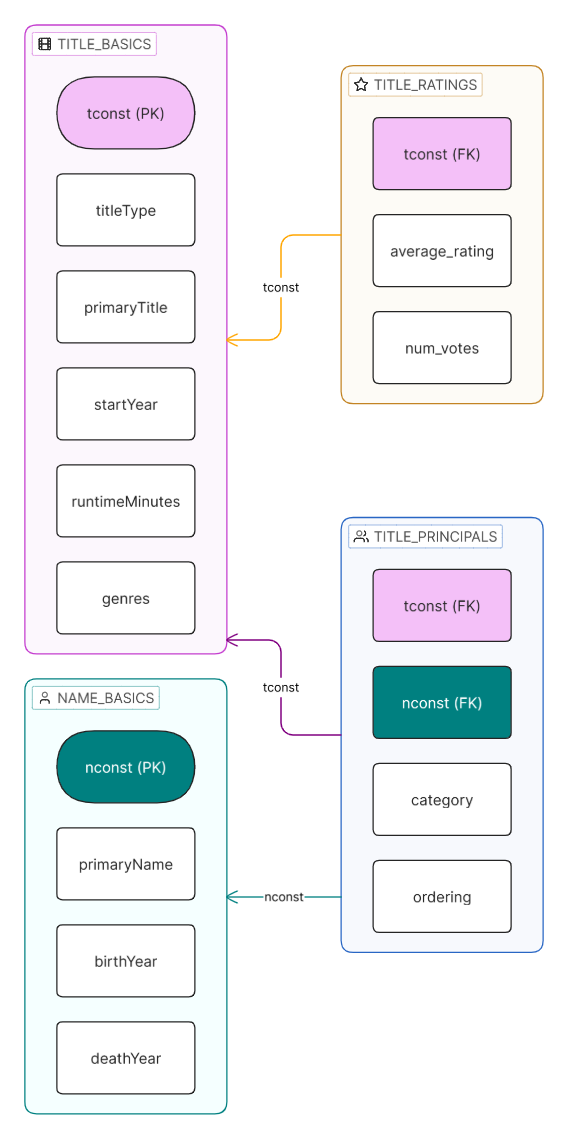
\includegraphics[width=\textwidth,height=0.75\textheight,keepaspectratio]{Report/graphs/imdb_er.png}
\caption{Entity-relationship diagram of the IMDB database schema. The \texttt{title\_principals} table acts as a central junction connecting titles to people, while \texttt{title\_ratings} provides aggregate user feedback per title. These relationships define the valid join paths for generated queries.}
\label{fig:imdb_schema}
\end{figure}

Table~\ref{tab:exp_config} summarizes the configuration parameters used across all experiments. These values were selected based on preliminary experiments and align with recommended settings from the MSCN literature. The pipeline is implemented in Python using PyTorch for the neural network training. PostgreSQL serves as the database backend, and Ollama\cite{Ollama2024} provides local LLM hosting. All experiments are executed on a standard workstation.

\begin{table}[tb]
\centering
\caption{Experimental configuration parameters.}
\label{tab:exp_config}
\begin{tabular}{|l|l|c|}
\hline
\textbf{Category} & \textbf{Parameter} & \textbf{Value} \\
\hline
\multirow{3}{*}{Query Generation} & Total queries & 5000 \\
 & LLM batch size & 20 \\
 & LLM model & Llama 3.2 \\
\hline
\multirow{2}{*}{Database} & Materialized samples & 1000 \\
 & Max retries & 2 \\
\hline
\multirow{4}{*}{Active Learning} & Strategy & Random Sampling / MC Dropout \\
 & Rounds & 10 \\
 & Acquisition batch size & 200 \\
 & MC Dropout passes ($T$) & 25 \\
\hline
\multirow{4}{*}{MSCN Training} & Hidden units & 256 \\
 & Learning rate & $10^{-4}$ \\
 & Epochs per round & 10 \\
 & Training batch size & 1024 \\
\hline
\end{tabular}
\end{table}

\FloatBarrier
\subsection{Evaluation Metrics}

Model performance was evaluated primarily using Q-error, which is the standard evaluation metric for learned cardinality estimation. Q-error measures the multiplicative difference between predicted and true query cardinalities and is defined as:

\[
Q\text{-}error = \max \left( \frac{\hat{y}}{y}, \frac{y}{\hat{y}} \right)
\]

where $\hat{y}$ denotes the predicted cardinality and $y$ the true cardinality.

Unlike absolute error metrics such as mean squared error, Q-error remains meaningful across workloads spanning multiple cardinality scales. This property is necessary because query cardinalities may range from highly selective queries returning only a few tuples to large joins producing millions of rows.

In addition to median Q-error, higher-percentile statistics such as p90 and p95 were also analyzed to evaluate robustness and tail-end estimation behavior.

\section{Query Generation Analysis}

\subsection{Workload Structural Analysis}

The structural composition of a query workload plays a central role in determining the effectiveness of learned cardinality estimators. Neural estimators such as MSCN do not learn database semantics directly; instead, they infer statistical relationships from the structural and predicate patterns present in the training corpus. Consequently, the quality of the generated workload strongly influences both the estimator’s prediction behavior on unseen queries and the effectiveness of the active learning process. A workload that captures a broad range of query structures and predicate selectivities therefore provides a stronger foundation for robust generalization across evolving query distributions.

A workload dominated by a narrow class of query templates can introduce significant bias during training. For example, a workload containing mostly single-table queries may allow the model to learn simple selectivity patterns while failing to capture the uncertainty introduced by multi-table joins. Similarly, workloads with limited predicate diversity may prevent the estimator from adequately modeling relationships between filtering conditions and result cardinalities. To avoid these issues, the query generation pipeline explicitly incorporates diversity-aware prompting constraints designed to encourage variation across multiple structural dimensions.

The following analysis evaluates whether the LLM-generated workload successfully captures the intended structural diversity relative to a synthetic reference distribution generated using rule-based random query construction techniques commonly employed in prior learned cardinality estimation benchmarks~\cite{leis2015how}. In particular, we examine distributions over query graph size, join complexity, predicate complexity, and resulting cardinality ranges. We additionally compare the generated workload against this synthetic baseline and quantify distributional similarity using KL divergence analysis.

Figure~\ref{fig:tables_compare} shows the distribution of table counts per query for both synthetic and LLM-generated workloads. In both cases, two-table queries form the dominant portion of the workload, while single-table and three-table queries remain well represented. However, the LLM-generated workload exhibits a slightly broader spread toward simpler query structures, indicating that the model naturally produces a mixture of lightweight and moderately complex relational patterns rather than converging to a single template.

\begin{figure}[tb]
\centering
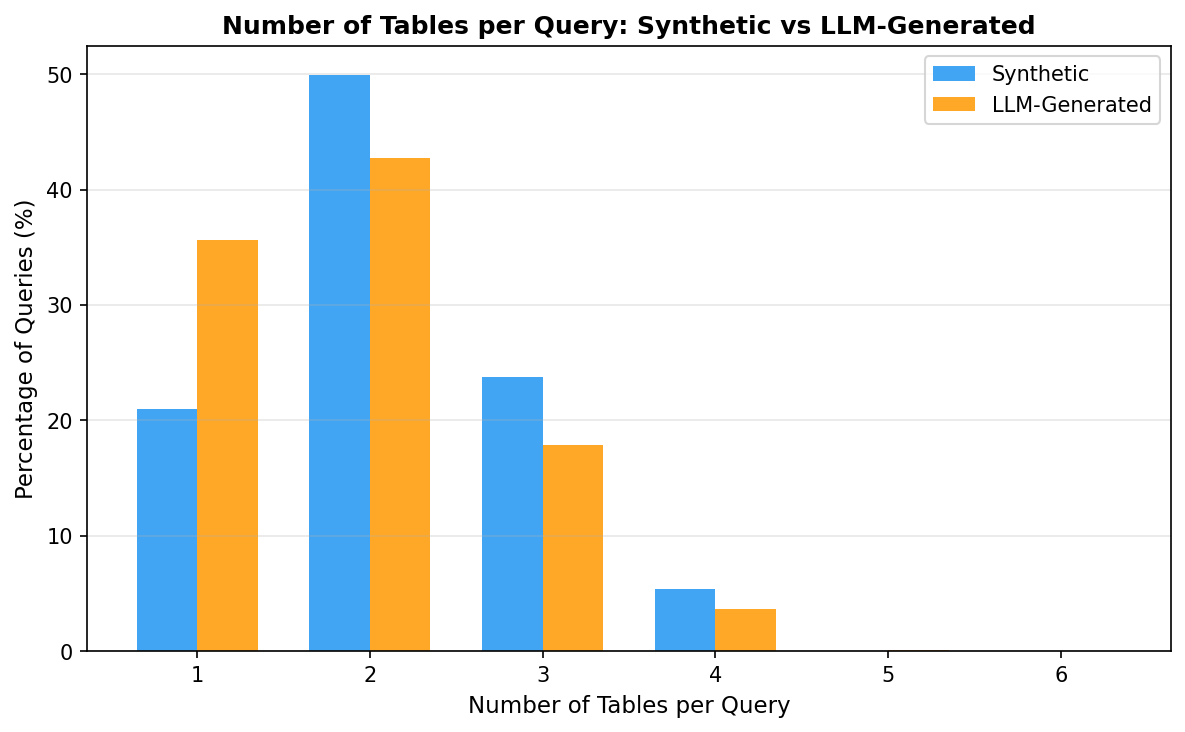
\includegraphics[width=0.8\textwidth]{Report/graphs/dist_tables.png}
\caption{Comparison of table-count distributions between synthetic and LLM-generated workloads. The LLM-generated workload preserves the overall structural balance while introducing additional variability in query graph size.}
\label{fig:tables_compare}
\end{figure}

Table-count distributions directly influence relational complexity during estimation. Single-table queries primarily evaluate predicate selectivity estimation, whereas multi-table queries require reasoning about join interactions and correlation effects. The observed distribution therefore indicates that the generated workload exposes the estimator to multiple levels of relational complexity rather than concentrating on a narrow subset of query structures.

Another notable observation is that the LLM-generated workload does not exactly reproduce the synthetic distribution. Instead, it introduces moderate deviations toward simpler structures. This behavior is desirable because it produces a mixture of both simple and complex query structures. A perfectly uniform distribution across all structural categories would not necessarily correspond to realistic database usage patterns.

Figure~\ref{fig:joins_compare} compares the distribution of join counts. Queries without joins correspond to single-table selections, whereas queries with one or more joins introduce increasingly complex relational interactions. The LLM-generated workload maintains a balanced distribution across these categories, demonstrating that the diversity prompting mechanism successfully prevents collapse toward only simple or only highly connected query structures.

\begin{figure}[tb]
\centering
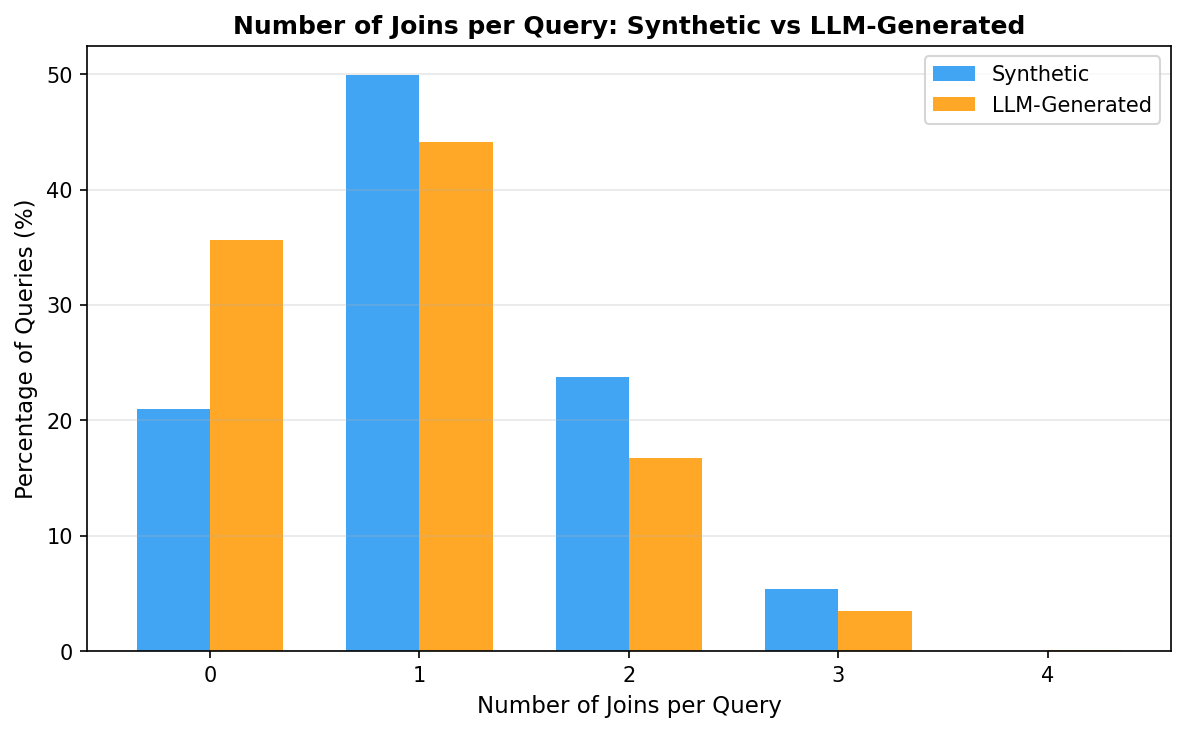
\includegraphics[width=0.8\textwidth]{Report/graphs/dist_joins.png}
\caption{Comparison of join-count distributions between synthetic and LLM-generated workloads. The generated workload spans both simple selection queries and multi-table join queries.}
\label{fig:joins_compare}
\end{figure}

Join operations are widely recognized as one of the primary sources of uncertainty in cardinality estimation. Errors introduced during join estimation often compound multiplicatively across execution plans, leading to poor join ordering decisions and inefficient query plans. For this reason, ensuring sufficient diversity in join structures is essential for training robust learned estimators.

The generated workload demonstrates consistent coverage across queries containing zero, one, and multiple joins. Queries without joins primarily capture base-table filtering behavior, while queries with one or more joins introduce additional dependencies between relations. These dependencies are challenging because traditional estimators often rely on independence assumptions that break down for correlated joins and predicates.

By incorporating a balanced mix of join complexities, the workload allows the model to observe both local predicate effects and broader relational interactions. This diversity is especially important for active learning, since informative samples are frequently concentrated near regions of high structural uncertainty, which commonly arise in multi-join queries.

Figure~\ref{fig:predicates_compare} presents the predicate count distribution. Most generated queries contain one or two predicates, while a smaller fraction includes more complex filtering conditions. Compared to the synthetic workload, the LLM-generated queries show a stronger concentration around low-to-moderate predicate counts, reflecting realistic query-writing patterns while still preserving diversity across selectivity regimes.

\begin{figure}[tb]
\centering
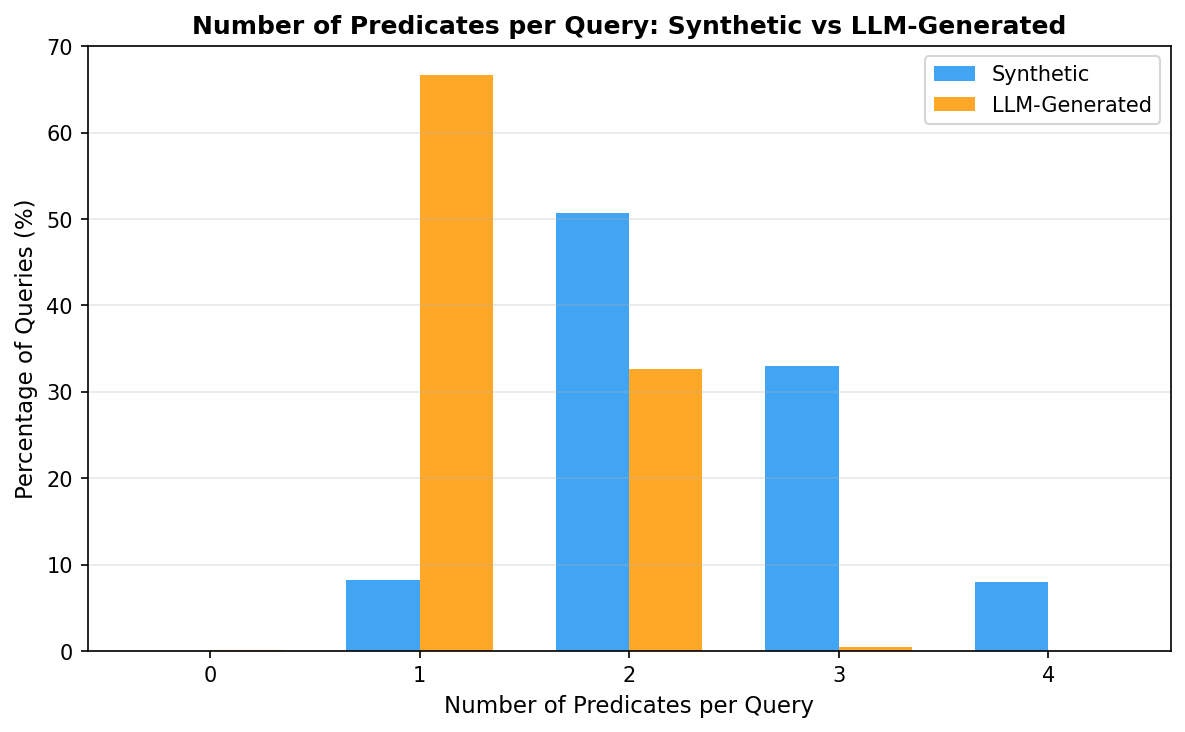
\includegraphics[width=0.8\textwidth]{Report/graphs/dist_predicates.png}
\caption{Comparison of predicate-count distributions between synthetic and LLM-generated workloads. The generated workload reflects diverse filtering complexity while maintaining structural diversity.}
\label{fig:predicates_compare}
\end{figure}

Predicate distributions provide insight into the selectivity characteristics of the workload. Predicate complexity influences workload selectivity characteristics and exposes the estimator to a broader range of filtering behaviors. Since MSCN represents predicates through learned set embeddings, exposure to diverse predicate combinations improves the model’s ability to capture non-linear relationships between filtering conditions and cardinality outcomes.

\subsection{KL-Divergence and Distributional Convergence}

While visual inspection of workload distributions provides qualitative evidence of structural diversity, a quantitative comparison is necessary to determine how closely the generated workload approximates the target synthetic distribution. To evaluate this similarity, we compute the Kullback--Leibler (KL) divergence between the feature distributions of the synthetic and LLM-generated workloads.

KL divergence measures the information loss incurred when one probability distribution is used to approximate another distribution\cite{lin2025playstyleartificialintelligenceinitial}. It is commonly used to compare distributional similarity in probabilistic modeling and behavioral alignment tasks~\cite{DBLP:journals/corr/abs-2503-24228}. In the context of workload generation, KL divergence provides a principled way to measure how closely the generated query corpus matches the intended workload characteristics.

Formally, the KL divergence between two discrete probability distributions $P$ and $Q$ is defined as:

\begin{equation}
D_{\mathrm{KL}}(P \parallel Q) = \sum_{i} P(i)\log \frac{P(i)}{Q(i)}
\end{equation}

where $P(i)$ represents the probability of observing feature value $i$ in the reference synthetic workload and $Q(i)$ represents the corresponding probability in the LLM-generated workload. Lower divergence values indicate stronger similarity between the two distributions, whereas larger values indicate greater structural mismatch.

In this work, KL divergence is computed independently for the distributions of tables, joins, and predicates. The metric is evaluated progressively as additional queries are generated, allowing us to analyze whether the workload converges toward the target structural characteristics over time.

\begin{figure}[tb]
\centering
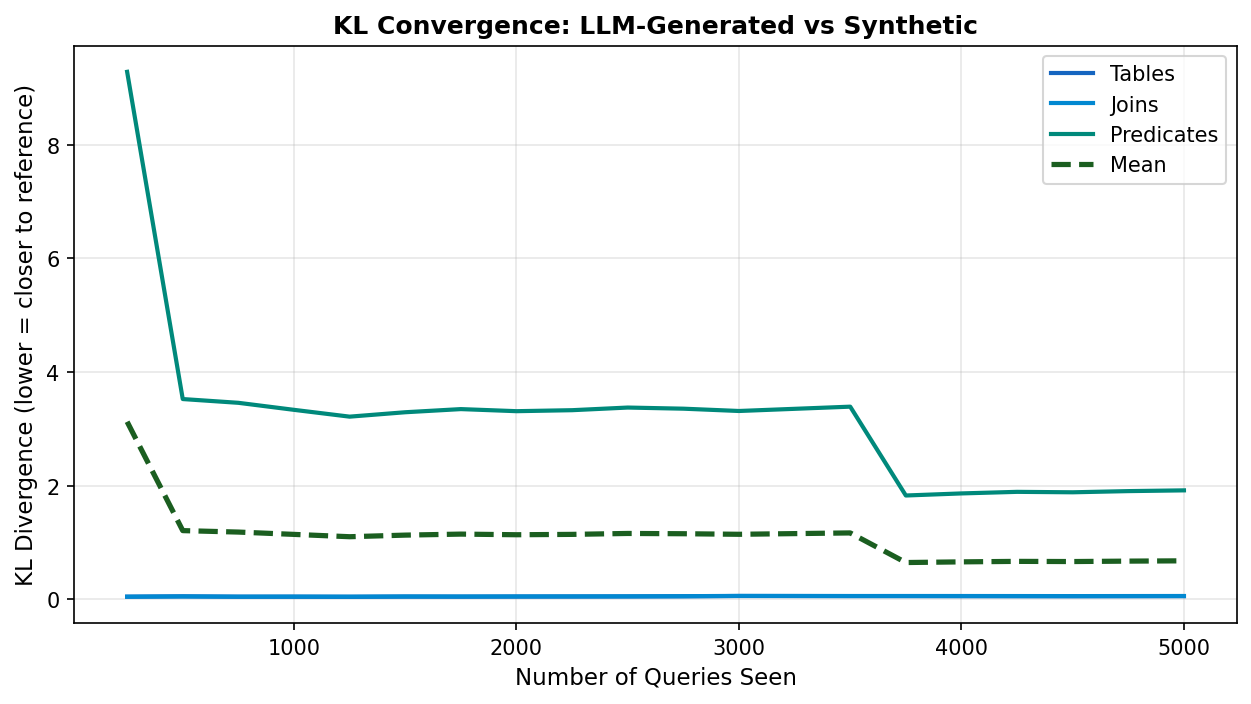
\includegraphics[width=0.9\textwidth]{kl_convergence.png}
\caption{KL-divergence convergence trends for tables, joins, predicates, and the aggregated mean between synthetic and LLM-generated workloads. Lower divergence values indicate stronger distributional similarity. The decreasing trends demonstrate progressive convergence toward the target workload characteristics as more queries are generated.}
\label{fig:kl_convergence}
\end{figure}

Figure~\ref{fig:kl_convergence} presents the KL-divergence trajectories for tables, joins, predicates, and the aggregated mean as the number of generated queries increases. Several important observations can be made from these convergence trends. A decreasing KL-divergence indicates that the generated workload distribution becomes increasingly similar to the target workload distribution over time. The table and join divergence curves remain near zero throughout the experiment and largely overlap visually due to their similarly low divergence values relative to the predicate distribution.

First, the divergence associated with table-count and join-count distributions decreases rapidly and stabilizes at relatively low values. This indicates that the LLM-generated workload successfully reproduces the overall structural composition of the reference workload, particularly with respect to query graph size and join complexity. The stability of these curves further suggests that the generation process does not collapse toward a narrow subset of repetitive query templates.

Second, predicate distributions exhibit higher divergence values compared to tables and joins. This behavior is expected because predicate generation involves greater combinatorial complexity. While table and join structures are constrained by the schema graph, predicate construction depends on combinations of columns, comparison operators, and value ranges, resulting in a significantly larger search space. Consequently, achieving convergence for predicate distributions requires a larger and more diverse query set.

Despite this increased variability, the predicate divergence demonstrates a clear downward trend as workload generation progresses. The aggregated mean KL divergence follows the same decreasing trajectory, indicating increasing similarity between the generated and reference workload distributions as additional queries are generated.

An important observation from Figure~\ref{fig:kl_convergence} is that divergence decreases more noticeably in the later stages of generation, after which the curves fluctuate within a lower range. This suggests that the workload generation process initially explores a broader structural space before gradually stabilizing around the target workload distribution. After this point, the divergence curves remain relatively stable, indicating that newly generated queries continue to preserve the desired workload characteristics rather than introducing excessive structural drift.

The convergence behavior observed in the KL-divergence analysis is particularly important for active learning. Active learning strategies rely on the availability of structurally diverse and statistically representative unlabeled samples. If the workload generation process produced highly repetitive or biased query structures, the acquisition function would repeatedly select similar queries, reducing the efficiency of uncertainty-driven sampling. The decreasing divergence trends therefore provide evidence that the generated workload maintains sufficient diversity while progressively aligning with the intended target distribution.

Overall, the KL-divergence analysis provides quantitative evidence that the proposed diversity-guided prompting strategy produces structurally stable and statistically representative workloads. Rather than repeatedly generating highly similar queries, the LLM progressively expands coverage across the workload feature space while maintaining alignment with the target structural distribution over time.

\begin{figure}[tb]
\centering
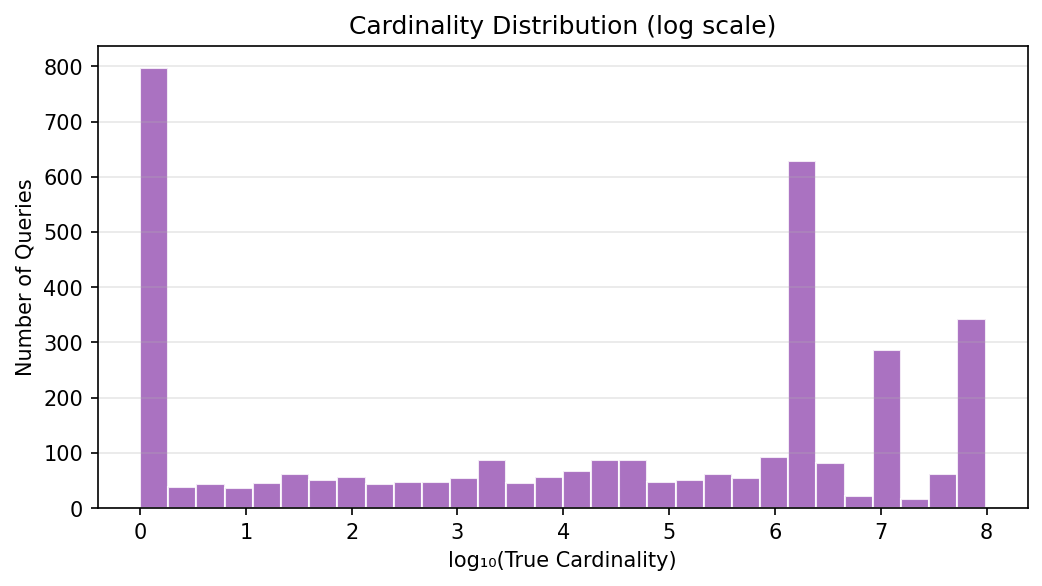
\includegraphics[width=0.85\textwidth]{data_cardinality_distribution.png}
\caption{Distribution of true query cardinalities on a logarithmic scale. The workload spans several orders of magnitude, exposing the estimator to both highly selective queries and large-scale scans.}
\label{fig:cardinality_dist}
\end{figure}

Finally, Figure~\ref{fig:cardinality_dist} shows the distribution of true query cardinalities on a logarithmic scale. The workload spans several orders of magnitude, ranging from highly selective queries returning only a few tuples to broad scans producing millions of rows. This long-tailed distribution is essential for training robust cardinality estimators, as it forces the model to learn accurate predictions across both sparse and dense selectivity regimes. The presence of such large variance also motivates the use of relative-error metrics such as Q-error, which remain meaningful across wide cardinality scales.

Overall, the workload analysis demonstrates that the generated query corpus captures substantial diversity across multiple orthogonal dimensions, including relational complexity, join structure, predicate composition, and selectivity behavior. This diversity is critical not only for supervised training but also for the effectiveness of active learning.

Furthermore, the convergence trends observed in the KL-divergence analysis suggest that the LLM-based generation process remains relatively stable as the workload grows. This is an important property for scalable workload generation because it indicates that increasing the query budget does not simply produce redundant templates, but instead incrementally improves coverage of the target workload distribution.

Taken together, these results validate the suitability of the generated workload for training learned cardinality estimators and provide empirical evidence that the proposed generation framework produces structurally rich and statistically representative query corpora.

\section{Active Learning and Model Training Results}

The workload diversity experiments presented in the previous section evaluate the structural properties of the LLM-generated query corpus. Due to the computational overhead associated with repeated query labeling and retraining, the controlled comparison between random sampling and MC Dropout acquisition strategies is conducted on synthetic workloads with predefined structural distributions.

In contrast, the subsequent labeling-efficiency and PostgreSQL comparison experiments are evaluated on LLM-generated workloads in order to assess the practical behavior of the proposed framework under automatically generated query distributions. This separation enables controlled analysis of active learning behavior while still evaluating the quality and executability of the LLM-generated workloads independently.

This section evaluates the effectiveness of the proposed active learning framework using workloads generated from synthetic query distributions. In particular, the experiments compare uncertainty-driven acquisition using MC Dropout against a standard random sampling baseline to determine whether uncertainty-aware query selection improves the efficiency, accuracy, and robustness of learned cardinality estimation.

The primary objective of active learning in this setting is to reduce the number of labeled training queries required to achieve strong estimation performance. Since obtaining query labels requires executing SQL queries against the underlying database system, labeling large workloads can be computationally expensive. An effective acquisition strategy should therefore identify the most informative queries for labeling, enabling the model to learn representative workload characteristics with fewer training samples.

The following analysis examines the learning behavior of the estimator across successive active learning rounds. In particular, we analyze convergence efficiency, prediction calibration, and the evolution of Q-error statistics under both random sampling and uncertainty-guided acquisition.

\subsection{Learning Efficiency Across Active Learning Rounds}

Figure~\ref{fig:learning_curve_comparison} compares the validation median Q-error achieved by random sampling and MC Dropout as the number of labeled synthetic queries increases. Both strategies exhibit a consistent reduction in validation error as additional labeled samples are incorporated into the training set, confirming that the estimator benefits from progressively larger workloads. However, the MC Dropout generally improves sample efficiency in this setup, but gains are not monotonic across rounds and can vary by run, seed, and workload sample.

\begin{figure}[tb]
\centering
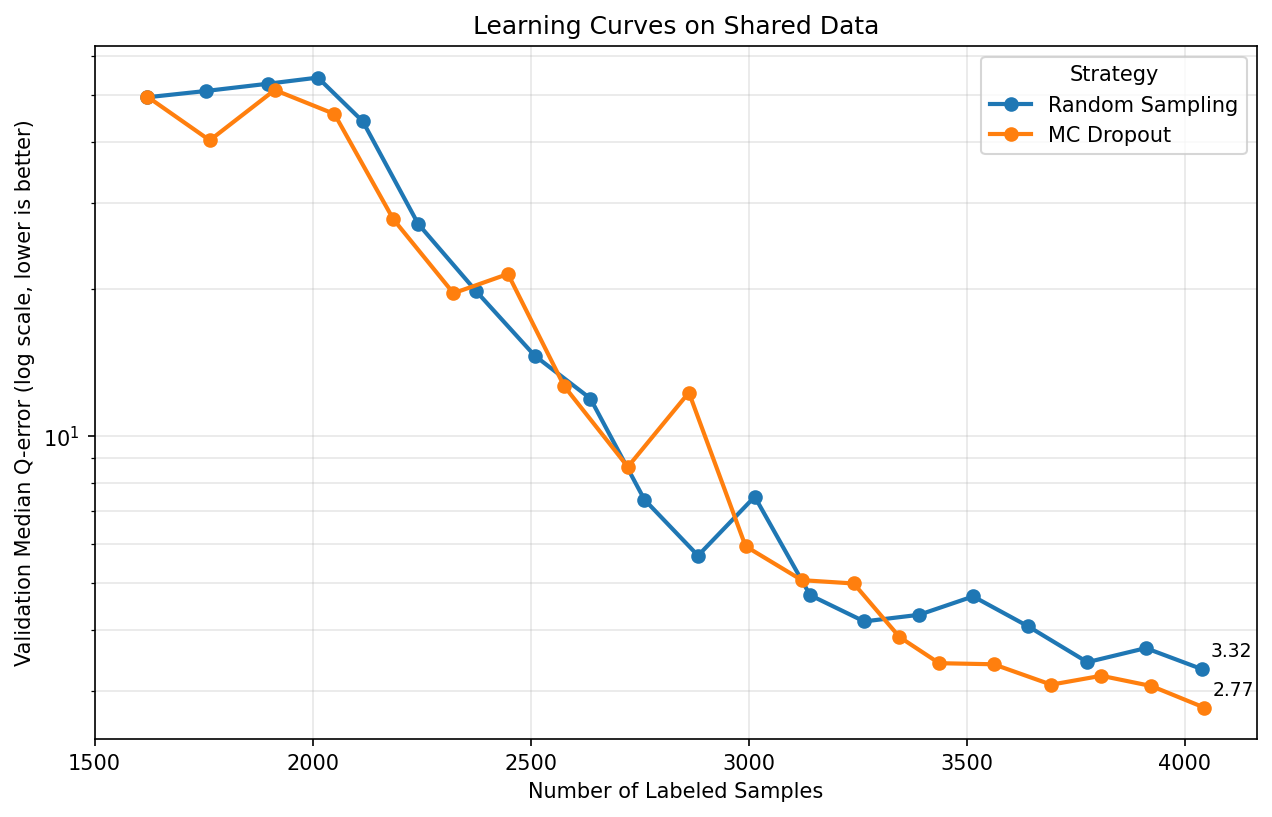
\includegraphics[width=0.9\textwidth]{Report/graphs/comparison_learning_curves.png}
\caption{Learning curves comparing random sampling and MC Dropout on synthetic query workloads. MC Dropout consistently achieves lower validation median Q-error with the same labeling budget, indicating improved sample efficiency during query acquisition.}
\label{fig:learning_curve_comparison}
\end{figure}

The difference between the two acquisition strategies becomes increasingly pronounced during later rounds of active learning. While the improvement achieved by random sampling gradually begins to plateau, MC Dropout continues reducing validation error. These findings suggest that uncertainty-aware query selection can reduce the labeling effort required to train learned cardinality estimators while maintaining strong performance on the evaluated workloads.

An important observation is the final performance gap between the two strategies. MC Dropout achieves lower validation median Q-error while using the same labeling \textbf{budget as random sampling}, demonstrating improved sample efficiency. From an active learning perspective, this result supports the hypothesis that uncertainty estimates can guide the acquisition process toward queries that provide greater learning benefit than randomly selected samples.

Most performance improvement occurs during the early acquisition rounds, indicating that uncertainty-guided selection rapidly identifies highly informative queries. The persistent gap between MC Dropout and random sampling further suggests that uncertainty estimates remain useful in later training stages.

Figure~\ref{fig:mc_dropout_curve} further illustrates the convergence behavior of the MC Dropout strategy using a workload configuration with 1,000 labeled queries. The validation median Q-error decreases sharply during the initial acquisition rounds before gradually stabilizing as the model approaches convergence. Overall, the active learning process achieves approximately 71.7\% reduction in median validation Q-error relative to the initial model within this setting.

\begin{figure}[tb]
\centering
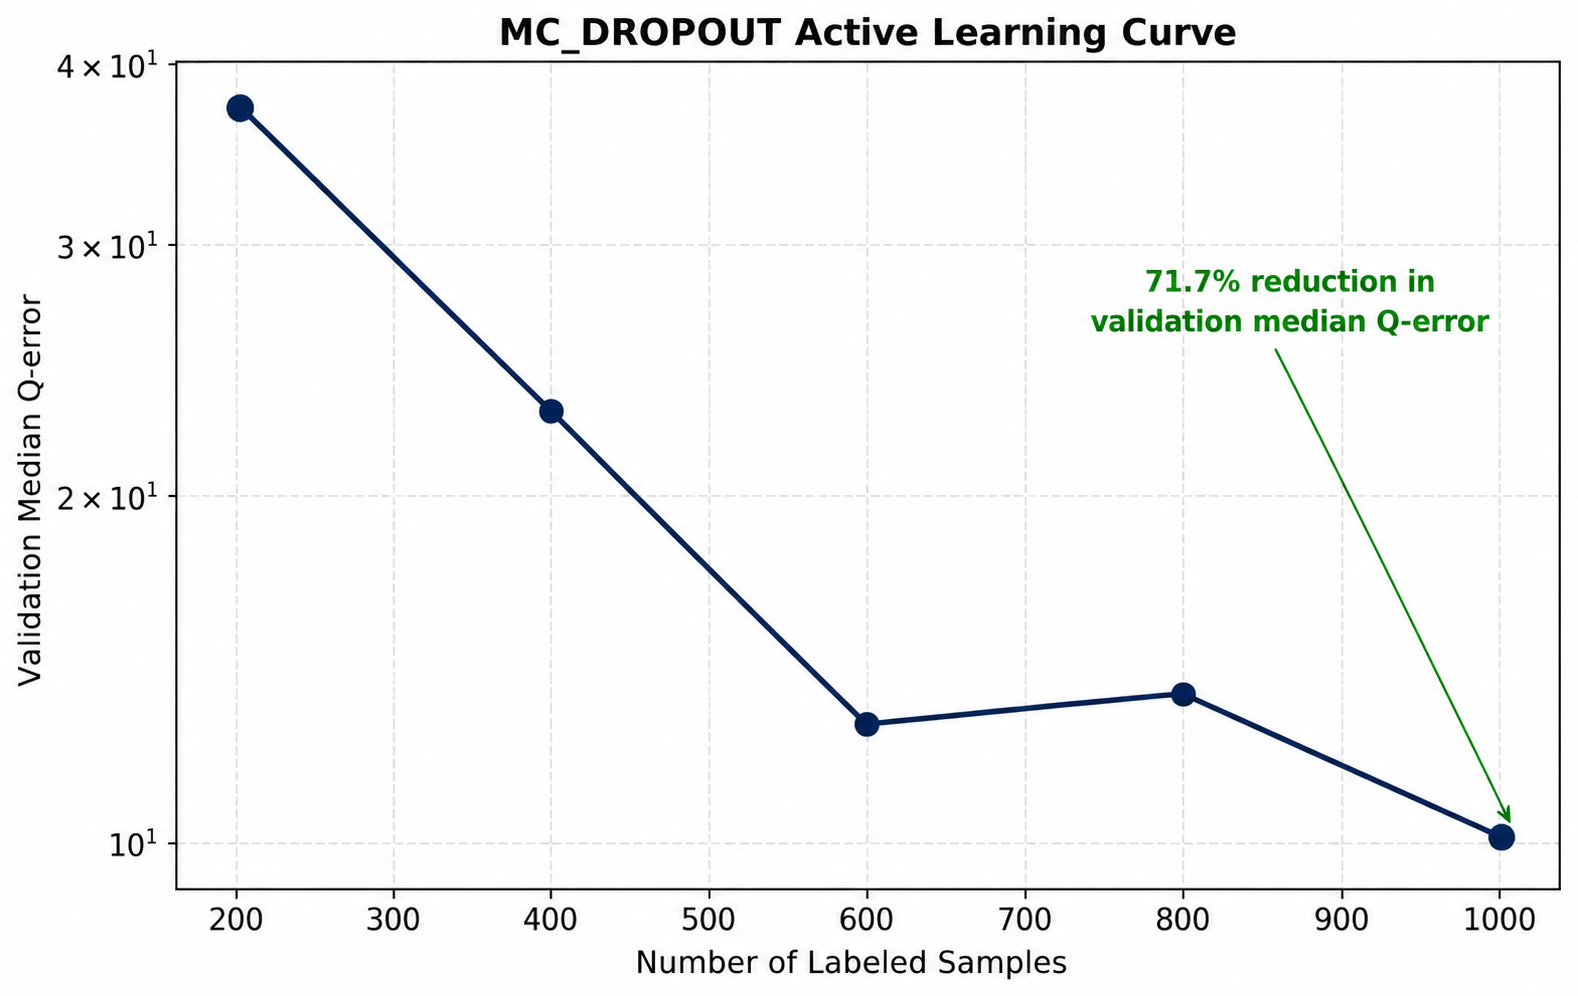
\includegraphics[width=0.75\textwidth]{train_learning_curve_mc_dropout.png}
\caption{MC Dropout active learning curve for the experimental configuration using 1,000 labeled queries. The reduction in validation median Q-error illustrates the convergence behavior of uncertainty-guided sample acquisition across active learning rounds.}
\label{fig:mc_dropout_curve}
\end{figure}

The steep decline during early rounds indicates that the model rapidly learns fundamental selectivity and join patterns from a relatively small set of informative synthetic queries before gradually approaching convergence.

\subsection{Prediction Accuracy and Calibration}

To evaluate prediction quality more directly, Figure~\ref{fig:predicted_vs_actual_comparison} compares predicted and actual cardinalities on a shared synthetic validation set. The plots are shown on logarithmic scales because query cardinalities span several orders of magnitude, ranging from highly selective queries to large-scale scans.

\begin{figure}[tb]
\centering
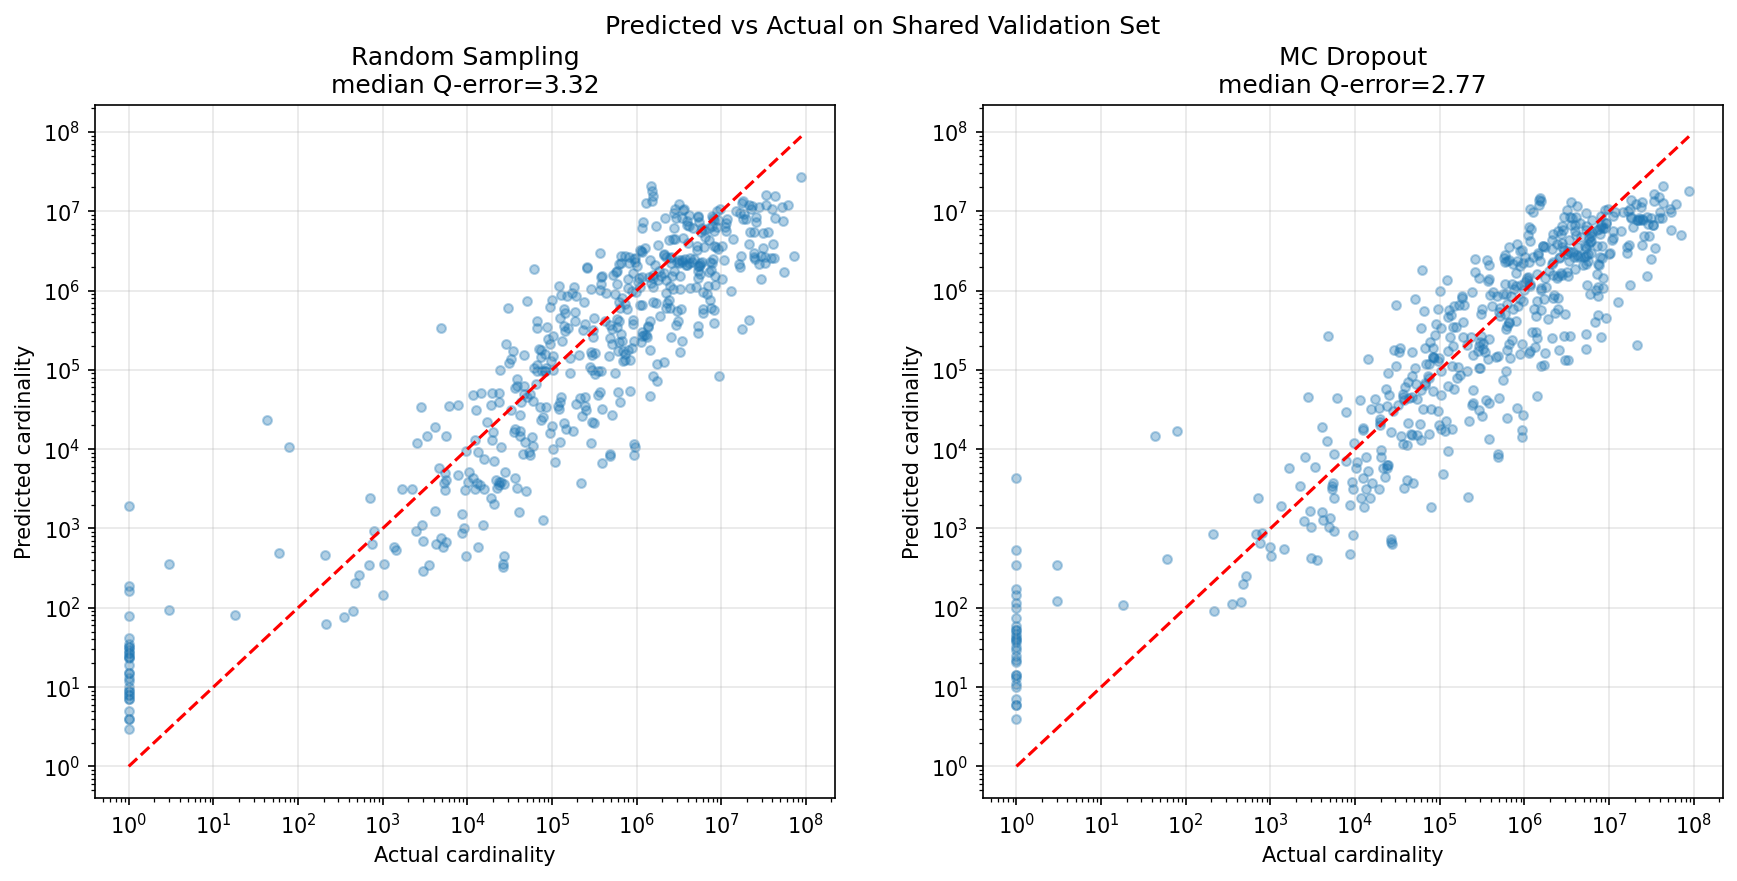
\includegraphics[width=\textwidth]{Report/graphs/comparison_predicted_vs_actual_scatter.png}
\caption{Predicted versus actual cardinalities for random sampling and MC Dropout on the shared synthetic validation set. Points closer to the diagonal line correspond to more accurate estimates. MC Dropout achieves tighter clustering around the diagonal and lower overall estimation error.}
\label{fig:predicted_vs_actual_comparison}
\end{figure}

Points located near the diagonal line correspond to accurate predictions, while deviations indicate estimation error. Both acquisition strategies successfully capture the overall trend of the validation workload, demonstrating that the MSCN estimator produces stable prediction behavior across multiple cardinality scales on the evaluated workload. However, the MC Dropout model exhibits visibly tighter clustering around the diagonal line, particularly for medium- and high-cardinality queries.

The reported median Q-errors further confirm this improvement. Random sampling achieves a median validation Q-error of 3.32, whereas MC Dropout reduces the median error to 2.77. This improvement suggests that uncertainty-guided acquisition improves estimation accuracy across the evaluated synthetic workload setup, demonstrating consistent gains over the baseline method.

Another important observation is that prediction dispersion increases toward the extreme ends of the cardinality spectrum. This behavior reflects the inherent difficulty of learned cardinality estimation, particularly for highly selective queries and extremely large joins where statistical correlations become increasingly difficult to model accurately. Despite these challenges, the MC Dropout strategy consistently produces estimates that remain closer to the ideal prediction line compared to the random baseline.

\subsection{Q-Error Distribution and Robustness Analysis}

While median Q-error provides a compact summary of estimation quality, analyzing higher-percentile errors provides additional insight into model robustness. Figure~\ref{fig:roundwise_qerror_stats} presents the evolution of median, 90th percentile (p90), and 95th percentile (p95) Q-errors across active learning rounds for both acquisition strategies. Lower median Q-error indicates improved average estimation quality, while reductions in upper-percentile errors indicate improved robustness against difficult outlier queries.

\begin{figure}[tb]
\centering
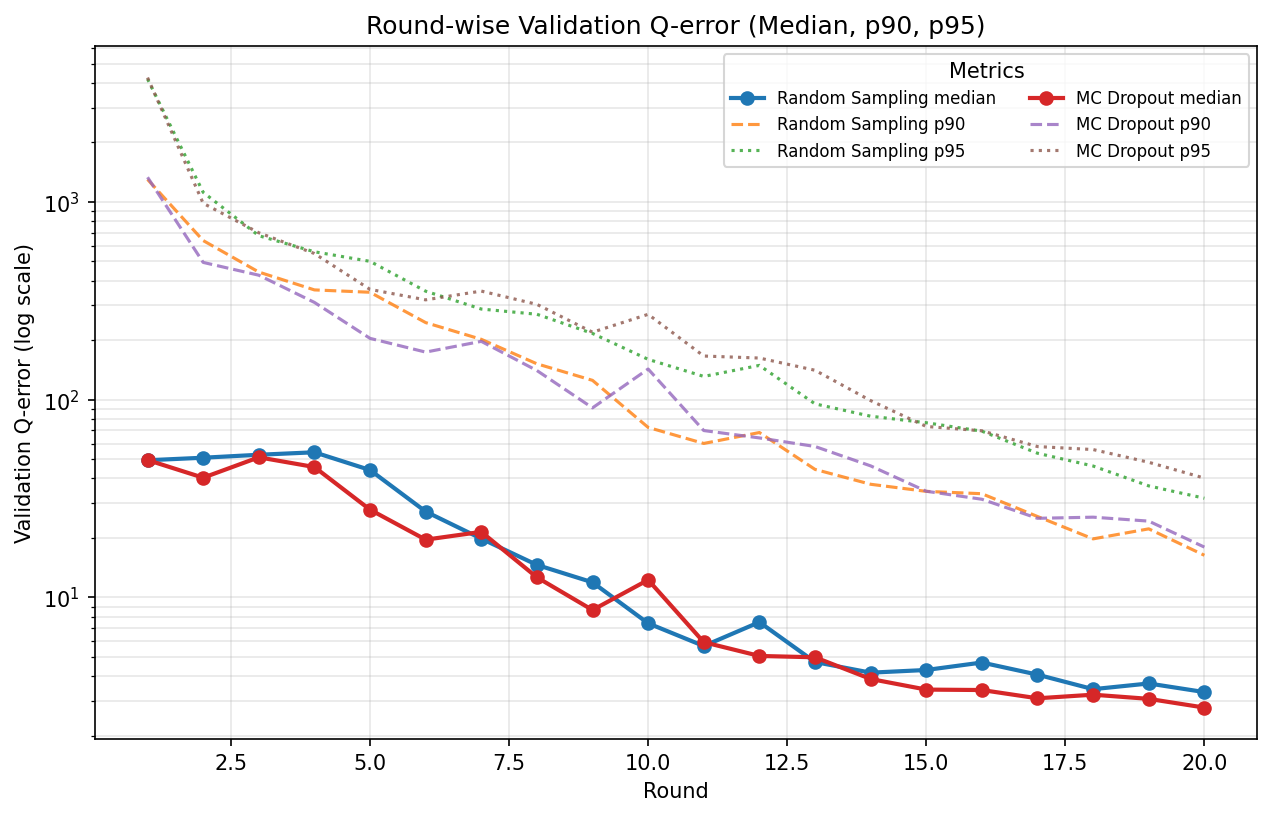
\includegraphics[width=0.95\textwidth]{Report/graphs/comparison_round_stats.png}
\caption{Round-wise validation Q-error statistics for random sampling and MC Dropout on synthetic workloads. The consistent reduction in median and tail-end errors demonstrates progressive improvement across active learning rounds.}
\label{fig:roundwise_qerror_stats}
\end{figure}

Several important trends emerge from this analysis. First, both acquisition strategies show substantial reductions in median Q-error as additional labeled queries are acquired over successive rounds. This confirms that active learning progressively improves the estimator’s ability to model workload selectivity patterns and join relationships.

Second, MC Dropout achieves consistently lower or comparable percentile errors across most rounds, particularly during later stages of training. The improvement is especially noticeable for the p90 and p95 metrics, which capture tail-end estimation behavior. 
Reducing extreme estimation errors is important because such failures can propagate through execution plans and negatively affect downstream optimization decisions.

Another important observation is the gradual stabilization of the percentile curves during later rounds. As the training workload becomes increasingly representative, the model approaches convergence and additional labeled queries provide smaller incremental improvements. This behavior is consistent with the convergence dynamics observed earlier in the learning curves.

The decreasing tail-end errors further indicate that uncertainty-guided acquisition improves not only average-case estimation quality but also robustness on difficult queries. By prioritizing uncertain or poorly modeled queries during acquisition, MC Dropout progressively reduces gaps in the model’s understanding of the workload distribution.

Overall, the experimental results demonstrate that MC Dropout provides a more effective active learning strategy than random sampling for synthetic query workloads. Compared to random acquisition, uncertainty-guided sampling achieves faster convergence, lower validation error, and stronger robustness across multiple evaluation metrics. These findings indicate that uncertainty-aware query selection improves sample efficiency and estimation robustness within the evaluated synthetic workload setting.

\section{Labeling Efficiency Analysis}

One of the primary motivations for incorporating active learning into the training pipeline is the high computational cost associated with obtaining query cardinality labels. Each labeled sample requires executing the corresponding SQL query against the database engine, which can become prohibitively expensive when training workloads contain thousands of queries. Consequently, reducing the number of required database executions is critical for improving the practical scalability of learned cardinality estimation systems.

The proposed active learning framework addresses this challenge by selectively labeling only the most informative queries rather than uniformly labeling the entire workload. Instead of treating all unlabeled queries as equally valuable, uncertainty-guided acquisition prioritizes samples that are expected to provide the greatest improvement to the estimator.

Figure~\ref{fig:labeling_efficiency} compares the labeling effort required by the active learning pipeline against a fully supervised baseline. The results demonstrate that the active learning approach achieves competitive estimation accuracy \textbf{while labeling only a fraction of the total query pool}. This reduction in labeling effort directly translates into lower execution overhead, reduced training time, and improved scalability for large workloads.

\begin{figure}[htbp]
\centering
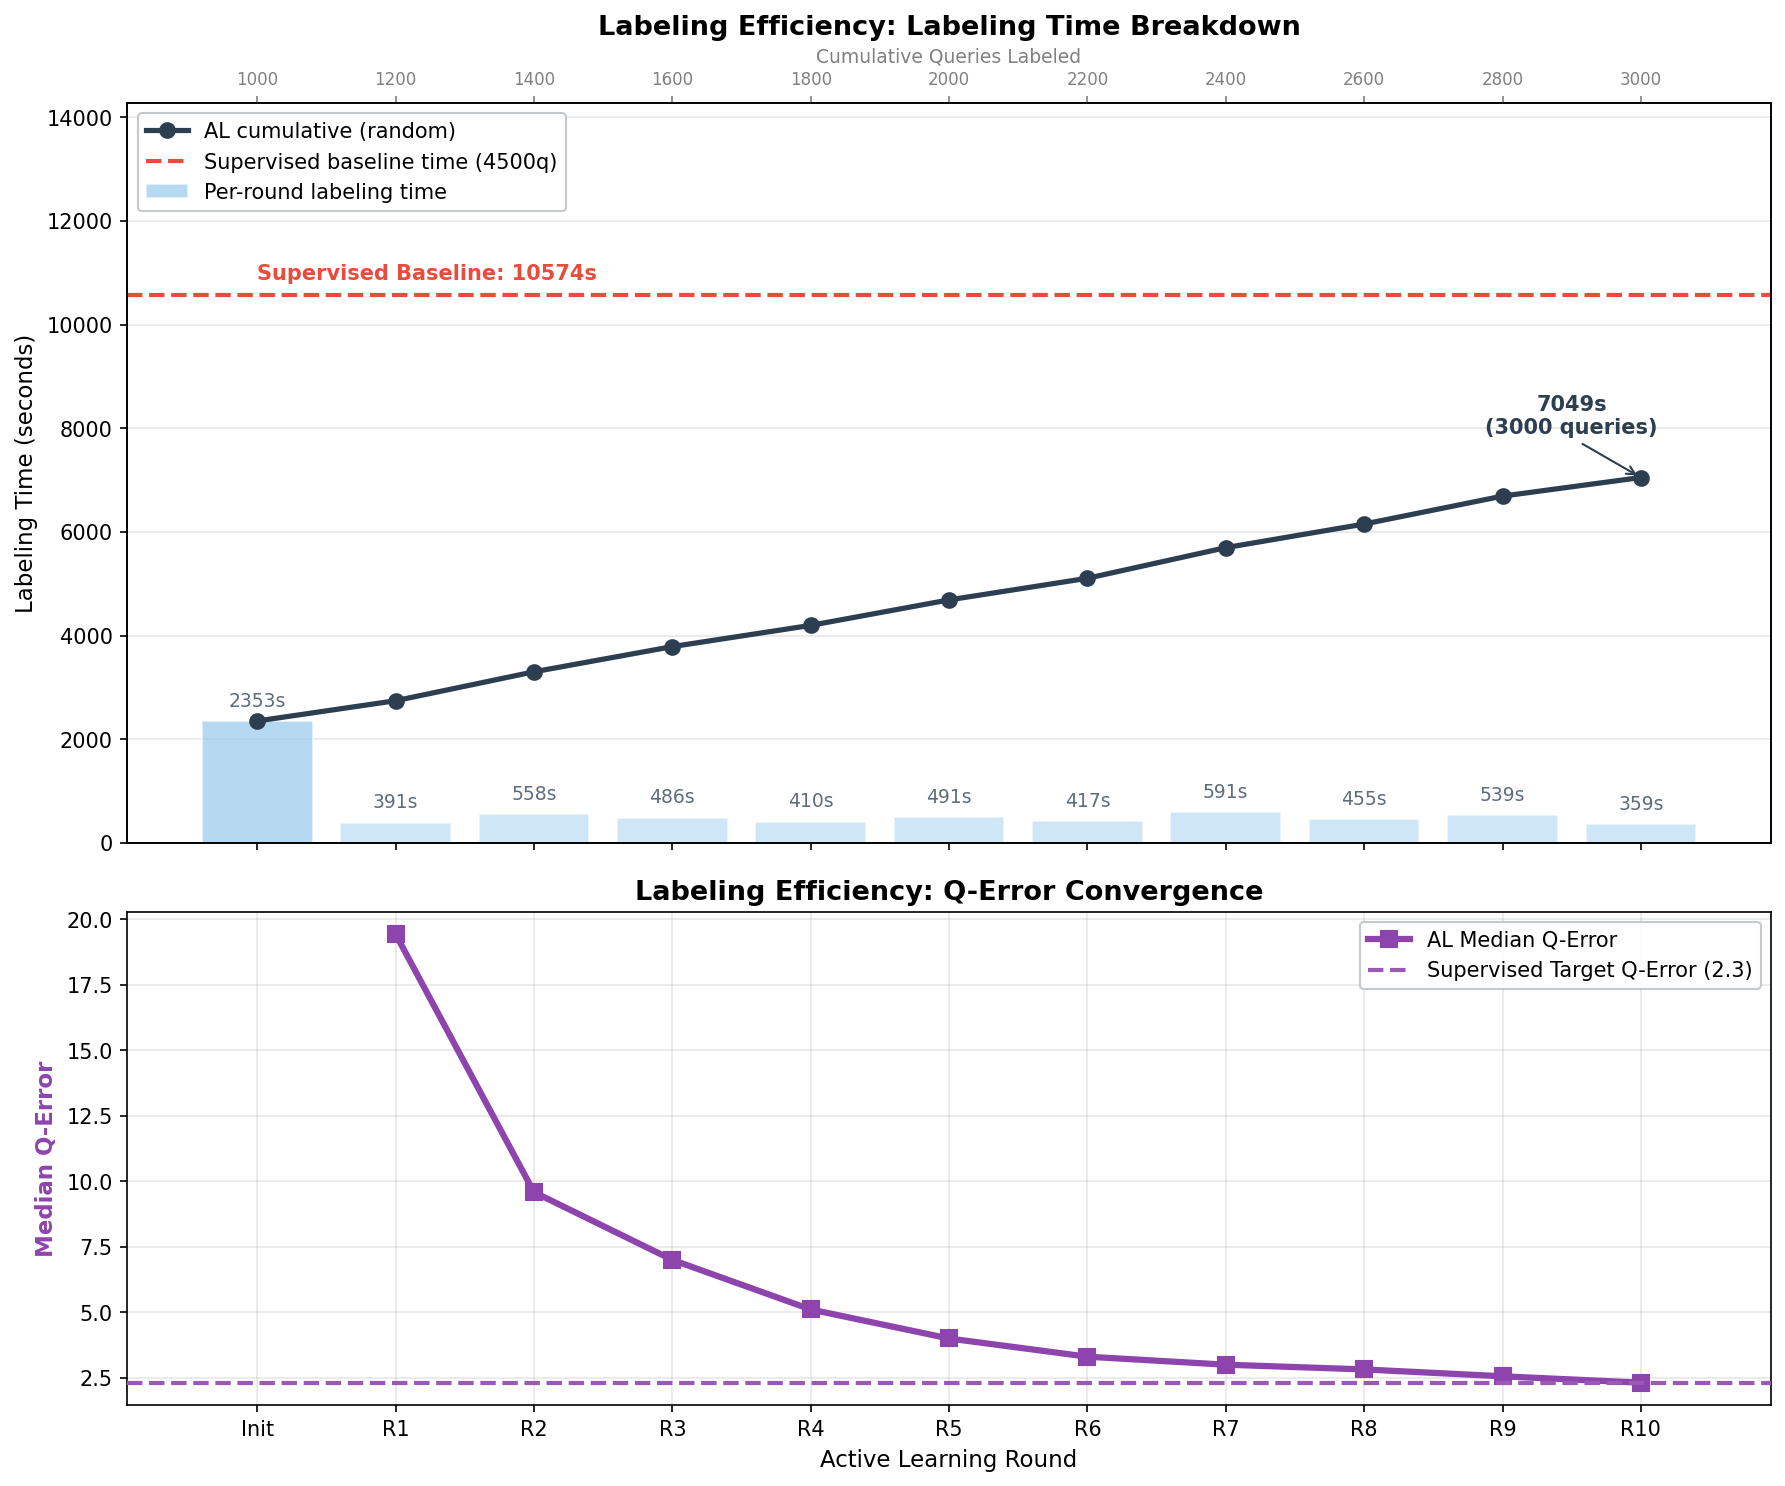
\includegraphics[width=\textwidth]{analysis_labeling_efficiency.png}
\caption{Labeling efficiency comparison between active learning and full supervision. The active learning framework achieves competitive estimation accuracy while requiring significantly fewer labeled queries, reducing the dominant execution cost in the training pipeline.}
\label{fig:labeling_efficiency}
\end{figure}

These results suggest that selectively labeling informative queries provides substantially greater learning benefit than uniformly expanding the labeled workload. By focusing labeling resources on uncertain or poorly modeled queries, the active learning framework extracts substantially more learning value per database execution than random or exhaustive labeling approaches.

This improvement is particularly important for learned cardinality estimation because workload labeling is often the dominant computational bottleneck in the training pipeline. Large analytical queries may require substantial execution time, especially when generating workloads spanning diverse join structures and selectivity conditions. Reducing the number of required executions therefore improves not only computational efficiency but also the practical feasibility of retraining estimators as database contents evolve over time.

Figure~\ref{fig:labeling_rate} further analyzes the robustness of the labeling pipeline by reporting the proportion of generated queries that were successfully labeled within the configured execution constraints.

\begin{figure}[htbp]
\centering
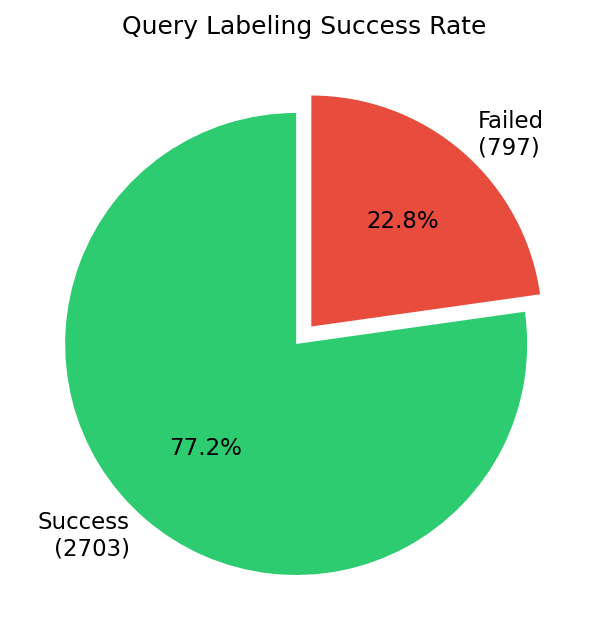
\includegraphics[width=0.85\textwidth]{analysis_labeling_rate.png}
\caption{Queries exceeding timeout limits or failing after retries are retained using a fallback cardinality value, so the pipeline can continue without dropping samples. As a result, the labeling outcome should be interpreted as successful executions versus fallback-labeled cases, not strict inclusion versus exclusion. The high success rate demonstrates that the generated queries remain largely executable within practical execution constraints.}
\label{fig:labeling_rate}
\end{figure}

Queries that exceed the database timeout threshold or repeatedly fail during execution are excluded from the final labeled workload. Such failures may arise from excessively expensive join plans, execution instability, or resource limitations within the database system. Despite these challenges, the labeling pipeline achieves a high overall success rate, indicating that the generated LLM workloads remain largely executable within realistic execution limits.

The high labeling success rate also provides indirect evidence that the workload generation framework produces largely executable queries. Since the generated queries are overwhelmingly executable and produce valid cardinality labels, the diversity-guided prompting strategy successfully balances structural complexity with practical executability. This balance is essential because excessively complex or pathological queries would reduce labeling throughput and limit the usefulness of the generated workload for active learning.

Overall, the labeling efficiency analysis demonstrates that active learning substantially reduces the execution cost associated with workload labeling while maintaining strong estimator performance. These results suggest that uncertainty-guided query acquisition can reduce labeling cost while maintaining strong estimation performance on diverse query workloads.

\section{Comparison with PostgreSQL Optimizer}

To further evaluate the effectiveness of the learned estimator, we compare its cardinality predictions directly against those produced by PostgreSQL’s native query optimizer. PostgreSQL relies primarily on histogram statistics and independence assumptions when estimating query cardinalities, whereas the MSCN model learns statistical relationships directly from query workloads and execution results.

This comparison is particularly important because cardinality estimation quality directly influences downstream query optimization decisions, including join ordering, operator selection, and memory allocation. Even moderate estimation errors can propagate through execution plans and significantly degrade query performance. Consequently, demonstrating improvements over the native PostgreSQL estimator provides evidence of the effectiveness of the proposed learned approach on the evaluated workload.

Figure~\ref{fig:pg_line} compares the distribution of Q-error values across query quantiles for PostgreSQL and the MSCN estimator on the shared validation workload. The evaluation in this section is conducted on the LLM-generated validation workload described earlier in the chapter.

\begin{figure}[tb]
\centering
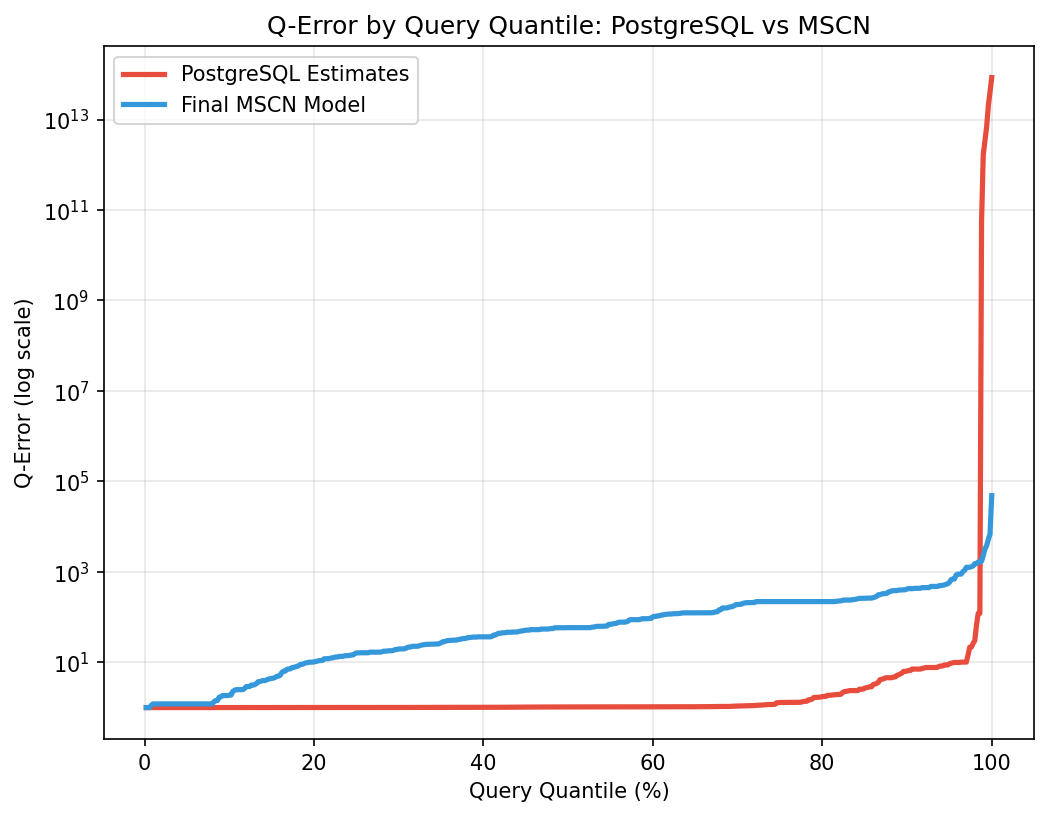
\includegraphics[width=\textwidth]{Report/graphs/compare_pg_vs_mscn_qerror_line.png}
\caption{Q-error by query quantile for PostgreSQL and the MSCN estimator on the validation workload. Lower curves indicate more accurate cardinality estimates across the evaluated query distribution, while steep increases near the upper quantiles reflect difficult outlier queries with large estimation errors.}
\label{fig:pg_line}
\end{figure}

The percentile-based comparison reveals substantially different error characteristics between the two estimators. PostgreSQL maintains relatively low Q-error values across most of the workload but exhibits extremely large estimation failures in the highest query quantiles, where Q-error increases abruptly by several orders of magnitude. In contrast, the MSCN estimator produces higher median error throughout much of the distribution but avoids the catastrophic outlier behavior observed in PostgreSQL. This suggests that the learned estimator achieves more stable worst-case behavior while sacrificing some accuracy on simpler query instances.

The sharp error escalation near the upper quantiles highlights structurally difficult queries involving highly selective predicates, sparse joins, or complex correlation patterns. Such queries challenge traditional histogram-based estimators because estimation errors propagate multiplicatively across join operations. The smoother MSCN error profile indicates more consistent generalization under these challenging conditions, even though its average estimation accuracy remains less competitive on easier portions of the workload.
\begin{figure}[tb]
\centering

\includegraphics[width=\textwidth]{compare_pg_vs_mscn_scatter.png}
\caption{Predicted versus actual cardinalities for PostgreSQL and MSCN. Points closer to the diagonal line correspond to more accurate cardinality estimates.}
\label{fig:pg_scatter}
\end{figure}

Across most query percentiles, PostgreSQL achieves lower Q-error than the MSCN estimator, indicating more accurate cardinality estimates for a large portion of the evaluated workload overall. This behavior is expected because the evaluated queries largely follow relatively simple predicate and join structures that align well with PostgreSQL’s histogram-based estimation framework. However, PostgreSQL also exhibits severe estimation failures in the highest query quantiles, whereas the MSCN estimator produces a comparatively smoother error profile with fewer catastrophic outliers. These results suggest that the learned estimator captures workload-dependent correlations and selectivity patterns that are difficult to represent using traditional histogram-based estimation methods alone.

The advantage of the MSCN estimator becomes particularly important for complex multi-table queries and highly selective predicates, where traditional independence assumptions often break down in practice. By learning representations directly from workload behavior, MSCN is able to model dependencies between predicates and joins more effectively than traditional histogram-based estimation methods.

Figure~\ref{fig:pg_scatter} provides visualization by comparing predicted and actual query cardinalities on a logarithmic scale. Points located near the diagonal line correspond to accurate predictions, while larger deviations indicate estimation error.

The MSCN predictions exhibit a comparatively smoother distribution of estimation errors across different cardinality ranges, while PostgreSQL demonstrates larger deviations for a small subset of difficult queries. These difficult cases are likely associated with correlated predicates or sparse join patterns that are challenging for traditional histogram-based estimation methods.

Another important observation is that the learned estimator maintains improved accuracy even at the extremes of the cardinality spectrum. Estimating very small or very large cardinalities is particularly challenging because such queries often correspond to sparse or highly correlated regions of the workload distribution. The improved stability of MSCN in these regions demonstrates the benefit of workload-driven learning for capturing complex statistical relationships.

Overall, the comparison with PostgreSQL demonstrates that traditional histogram-based estimation remains highly effective for a large portion of the evaluated workload, particularly for simpler query structures and predicates. However, the learned MSCN estimator exhibits more stable behavior on difficult outlier queries and complex selectivity patterns where traditional independence assumptions become less reliable. These results suggest that workload-driven learned estimators can complement traditional optimizer statistics, particularly for challenging query distributions involving sparse joins and correlated predicates.

\section{Discussion}

This chapter evaluated the proposed active learning framework across multiple dimensions, including workload diversity, labeling efficiency, estimation accuracy, and robustness. The experimental results demonstrate that the proposed framework produces structurally diverse LLM-generated query workloads and that uncertainty-guided acquisition improves learning efficiency on the evaluated synthetic workloads.

Beyond the quantitative improvements observed in validation Q-error and workload coverage, the experiments also provide broader insights into the behavior of learned cardinality estimation systems and the practical trade-offs involved in building scalable data-driven query optimizers. 

\subsection{Active Learning and Workload Diversity}

The experimental results demonstrate that uncertainty-guided acquisition improves labeling efficiency by prioritizing informative queries rather than uniformly sampling the workload. Queries associated with high predictive uncertainty typically correspond to regions of the workload distribution that are underrepresented or poorly modeled by the current estimator.

The learning curves indicate rapid improvement during early acquisition rounds followed by gradual convergence as the estimator observes increasingly representative workload patterns.

An important implication of these findings is that query quality is more important than query quantity during training. A relatively small but carefully selected labeled workload can provide comparable learning benefit to substantially larger randomly labeled datasets. This observation highlights the practical value of uncertainty-guided acquisition for reducing database execution overhead while maintaining strong estimation accuracy.

The quality of a learned cardinality estimator depends heavily on the diversity of the workload used during training. If the workload contains highly repetitive query structures or narrow selectivity patterns, the estimator may overfit to a limited subset of query templates and fail to generalize to unseen workloads.

The workload generation strategy proposed in this thesis addresses this challenge through diversity-guided prompting and structural constraint mechanisms. Rather than generating queries independently without feedback, the LLM is continuously guided using workload statistics such as table counts, join distributions, predicate frequencies, and cardinality ranges.

The workload analysis indicates that the proposed generation framework maintains broad workload coverage while progressively converging toward the target workload distribution. This balance between diversity and distributional stability is particularly important for active learning because it provides heterogeneous unlabeled samples without collapsing toward repetitive query templates.

An important observation from the KL-divergence analysis is that predicate distributions converge more slowly than join or table distributions. A likely explanation is that predicate construction involves significantly greater combinatorial complexity. While table and join structures are constrained by the schema graph, predicates depend on combinations of columns, operators, and value ranges, resulting in a much larger structural search space.

Despite this increased variability, the workload generation process avoids collapsing toward overly repetitive query structures. This behavior is particularly important because active learning fundamentally relies on the availability of sufficiently diverse unlabeled samples for effective learning. If the generated workload lacked sufficient structural variation, the acquisition process would provide only limited additional information in later rounds, thereby reducing its overall effectiveness.

The results therefore reinforce the importance of workload diversity for learned cardinality estimation. The value of LLM-based workload generation lies not only in automating SQL query creation but also in enabling broader structural exploration than would be feasible using manually designed templates alone.

\subsection{Practicality and Scalability of the Pipeline}

Another important contribution of this work is the development of a fully automated pipeline for workload generation, labeling, and model training. Traditional workload construction often requires significant manual effort, including hand-written query templates, schema-specific heuristics, and extensive tuning for each database environment.

The proposed framework reduces this manual dependency by leveraging LLM-guided workload generation combined with automated validation and labeling stages. Because the pipeline relies primarily on schema metadata and workload statistics, it remains largely schema-independent within the supported query fragment and adaptable to relational schemas with defined join relationships.

The modular architecture of the system also improves reproducibility and experimentation efficiency. Individual components such as workload generation, query validation, uncertainty acquisition, labeling, and training can be modified independently without redesigning the entire pipeline. This flexibility simplifies experimentation with alternative acquisition strategies, model architectures, and workload configurations.

Another practical advantage is the reduction in engineering overhead associated with maintaining manually curated query workloads. Once schema information is extracted, the pipeline can continuously generate new training queries with minimal human intervention. This capability becomes increasingly valuable in dynamic environments where workloads evolve over time and estimators require periodic retraining.

The high query validation and labeling success rates observed during experimentation further demonstrate that the automated generation strategy successfully balances workload diversity with practical executability. The majority of generated queries remain executable within the configured timeout limits, indicating that the workload generation process generally avoids excessively expensive query structures.

Although active learning improves labeling efficiency, it also introduces additional computational overhead compared to traditional supervised learning pipelines. In particular, uncertainty estimation using MC Dropout requires multiple stochastic forward passes through the model during acquisition. This increases inference cost relative to random query selection.

Another source of overhead arises from workload preprocessing and bitmap generation. The MSCN representation relies on sampled bitmap features to capture predicate selectivity information, and generating these features requires additional preprocessing during workload construction.

However, the experimental results suggest that these overheads are acceptable relative to the cost of exhaustive query labeling. Database execution remains the dominant computational bottleneck in the pipeline, particularly for complex analytical queries involving multi-way joins and large cardinalities. Reducing the number of required labeled queries therefore provides substantially greater computational savings than the additional inference cost introduced by uncertainty estimation.

An important trade-off also exists between workload diversity and execution efficiency. More structurally diverse workloads improve estimator generalization but may also increase the probability of generating expensive or difficult-to-execute queries. The validation and timeout filtering stages are therefore essential for ensuring that the final workload remains practically executable while preserving sufficient structural diversity.

Overall, the results suggest that uncertainty-guided active learning provides a balance between computational overhead and labeling efficiency. The additional acquisition cost introduced by MC Dropout is outweighed by the reduction in expensive database executions required to train an accurate estimator.

\subsection{Sources of Estimation Error}

Despite the overall improvement achieved by the learned estimator, several sources of estimation error remain challenging. One major difficulty arises from highly selective queries and extremely large joins, where sparse or skewed data distributions make accurate estimation inherently difficult.

Another important challenge involves unseen predicate combinations and rare join patterns that are poorly represented within the training workload. Although the diversity-guided generation strategy improves structural coverage, it is still difficult to exhaustively explore the enormous combinatorial space of possible SQL queries.

Prediction errors may also arise from limitations of the sampled bitmap representation used by MSCN. Bitmap samples provide only an approximate representation of predicate selectivity and may fail to capture fine-grained correlations within highly skewed datasets.

Workload shift represents an additional challenge for learned estimators. If the query distribution observed during deployment differs substantially from the workload used during training, model accuracy may degrade due to insufficient generalization. This limitation is particularly relevant in evolving database environments where application behavior changes over time.

Finally, the current workload generation framework focuses primarily on selection and join queries with relatively constrained SQL structure. More advanced SQL constructs such as nested subqueries, aggregations, window functions, and complex expressions are not extensively explored in the current implementation. Supporting these constructs would likely require more sophisticated workload generation and representation techniques.

\subsection{Implications for Learned Query Optimization}

The comparison with PostgreSQL highlights several important differences between learned and traditional cardinality estimation approaches. PostgreSQL primarily relies on histogram statistics, selectivity heuristics, and attribute independence assumptions when estimating query cardinalities.

While these techniques are computationally efficient, they often struggle to model correlations between predicates and joins, particularly for complex analytical workloads. As query complexity increases, estimation errors may accumulate throughout the execution plan and negatively affect downstream optimization decisions.

The experimental comparison suggests that workload-driven learned estimators are better able to capture complex predicate and join correlations than traditional statistics-based approaches on the evaluated workload. On the evaluated workload, PostgreSQL achieves lower Q-error over much of the distribution, while MSCN shows smoother tail behavior with fewer catastrophic outliers on difficult queries.

These findings suggest that workload-driven learned estimators can complement traditional query optimization pipelines, particularly in environments where complex workload correlations are difficult to capture using classical statistics.

The findings of this thesis have broader implications for the development of learned database systems and adaptive query optimizers. The results demonstrate that learned cardinality estimation can benefit substantially from automated workload generation and uncertainty-guided acquisition strategies.

One important implication is that the practical training cost of learned estimators depends not only on model architecture but also on the efficiency of the data acquisition process. Active learning provides a practical mechanism for reducing the dominant labeling cost while preserving estimator quality.

The integration of LLM-based workload generation further expands the feasibility of learned optimization pipelines by reducing the manual effort traditionally required to construct representative training workloads. As language models continue improving, automated workload generation may become increasingly capable of producing structurally diverse query distributions with minimal human supervision.

More broadly, the combination of learned estimation, uncertainty-guided acquisition, and automated workload generation illustrates how automated workload generation and adaptive acquisition strategies could support more self-adaptive learned database components capable of adapting continuously to evolving workloads. Such systems could dynamically acquire informative queries, retrain estimation models, and potentially improve optimization quality over time without requiring extensive manual intervention.

Overall, the results indicate that integrating automated workload generation with uncertainty-guided acquisition provides a practical framework for improving the scalability and labeling efficiency of learned cardinality estimation.

\section{Limitations and Threats to Validity}

Several limitations should be considered when interpreting the results presented in this thesis.

First, all experiments in this study were performed on the IMDB benchmark schema within a PostgreSQL environment. Although the proposed pipeline is designed to be largely schema-independent within the supported query fragment, the observed results may not directly generalize to substantially different schemas, database systems, or workload characteristics without additional evaluation.

Another limitation concerns workload realism. While the LLM-generated workloads exhibit structural diversity across joins, predicates, and selectivity ranges, they may not fully reflect real-world production query distributions. The generated workloads primarily consist of analytical \texttt{SELECT COUNT(*)} queries with constrained SQL structure and therefore do not capture the full complexity of operational database workloads.

The current implementation also focuses specifically on the MSCN architecture. Different learned cardinality estimation models may interact differently with active learning strategies and synthetic workload generation. As a result, the observed improvements cannot necessarily be assumed to transfer directly to alternative neural architectures without further experimentation.

Several practical constraints within the labeling pipeline may additionally influence the results. Ground-truth labels were obtained through database execution using timeout constraints and retry mechanisms. Queries exceeding the configured execution limits may either fail labeling or be retained with fallback labels, depending on the labeling path used. This can introduce label noise and should be considered when interpreting model accuracy and robustness. Similarly, bitmap-based representations provide only an approximate view of predicate selectivity and may not fully capture complex correlations or highly skewed data distributions.

Another important limitation concerns evaluation scope. The experiments primarily evaluate cardinality estimation quality using Q-error metrics. Although improved cardinality estimates are generally associated with better query optimization decisions, the experiments do not directly measure downstream effects on execution-plan quality, join ordering, or end-to-end query latency.

Finally, due to computational constraints, experiments were conducted using single training runs for each configuration. Neural network training and active learning may exhibit variability across random seeds and workload sampling processes. Future work should therefore evaluate the statistical robustness of the observed improvements across repeated experimental trials.